\documentclass[10pt,a4paper]{article}

\usepackage[utf8]{inputenc}
\usepackage[T1]{fontenc}
\usepackage{lmodern}
\usepackage{eso-pic}
\usepackage{transparent}
\usepackage{graphicx}

\newenvironment{figureH} {%
\begin{figure}[H]
}{%
\end{figure}
}

\title{ISE : Rendu 1}

\begin{document}

\maketitle

\section{Introduction}
Nous cherchons à calculer le pire temps de réponse de bout en bout dans un réseau où il n'y a pas de préemption lors du traitement des paquets à travers un noeud. Lors de la reception multiple de paquets, celui de priorité maximal est d'abord traité. Ce premier rendu décrit les résultats des calculs intermédiaires et donne une interprétation simple de l'exemple donné dans le cas d'étude et de son résultat.

\section{Description des données}
Le réseau est caractérisé par les données suivantes\\
$net=(\tau_i, P_i = [first_i,...,last_i], T_i, J_i, C_i^h, D_i, p_i, L_{min}, L_{max})$\\
%TODO decribe

Les données suivantes sont triavialement calculable\\
$first_{j,i}, last_{j,i}, slow_{j,i}, slow_i$\\
$hp_i, sp_i, lp_i$\\

Les calculs de $S_{min}$ et $S_{max}\\
$S_{max_i}^h = L_{max} \times (|[first_i ... h]| - 1) + \sum 
\limits_{h'=next(first_i)}^{h'=pre(h)}C_i^{h'}$ \\
$S_{min_i}^h = L_{min} \times (|[first_i ... h]| - 1) + \sum 
\limits_{h'=next(first_i)}^{h'=pre(h)}C_i^{h'}$ \\
$B_{i}^{slow}$ dépend de lui-même.\\

Les données suivantes peuvent-être calculées de manière paresseuse et ensuite rangées en mémoire pour ne pas avoir à les recalculer\\
For all h on path\\
$M_i^{h}$\\
For all node i, j\\
$A_{i,j}$\\

La donnée $\delta_i$ est difficile à calculer.\\

On calcule $R_{i,t}$ ensuite pour $t$ variant dans $[-J_i;-J_i+B_i^{slow}]$\\

Output\\
$R_{i} = max R_{i,t}$\\



\section{Calcul des données intermédiaires}
Dans cette section nous allons expliquer comment nous allons calculer les données 
intermédiaires en fonction des dépendances de donnés, ce qui nous facilitera la repartition 
des taches lors de l'implémentation.\\
Nous n'aborderons pas les dépendances avec les données initiales, car ces dernières sont stockées 
dans des structures de données adéquates et donc faciles d'accès.
Nous faisons aussi remarquer que le choix des structures de données fera 
l'objet d'un autre rendu.

\subsection{Données intermédiaires faciles à calculer}
Calcul de $A_{i,j}$ très simple, se résume à l'appel d'une fonction lorsque l'on a besoin de 
cette valeur\\
Calcul de $M_{i}^{first_{i,j}}$, très simple, se résume à l'appel d'une fonction.

\subsection{Données intermédiaires compliquées à calculer}

\subsubsection{Calcul de $B_i^{slow}$}
Ce calcul est compliqué car cette donnée dépend d'elle même dans une somme. Cependant 
nous remarquons que cette valeur ne peut être qu'un entier. Une première façon (un peu naïve) 
de la calculer est donc la suivante :\\
\linebreak
On part d'une valeur de $B_i^{slow} = 0$ et on effectue la boucle suivante :\\
Tant que $B_i^{slow} \neq \sum \limits _{j \in hp_i \cup sp_i \cup \{i\}} 
\lceil B_i^{slow}/T_ j\rceil$\\
\hspace{4em} incrémenter $B_i^{slow}$\\
Fin tant que\\
\subsubsection{Calcul de $\delta_i$}
Ce calcul est l'un des plus compliqué car il dépend du noeud sur lequel on 
travaille. En effet dans la formule donnée par l'article, ce calcul est composé 
d'une partie commune, puis d'une somme. Pour chaque noeud $h$ traversé 
(représenté par une itération dans la somme), il faut choisir la partie de la 
formule qui correspond au cas dans lequel on se trouve (cf. preuve de la 
Propriété 1, section 4.3 de l'article).

\subsubsection{Calcul de $W_{i,t}^{last_i}$}
Ce calcul dépend des calculs des 
$W$ des taches de priorités supérieures, stockées dans les structures de 
données définies à ce propos (pour ne pas avoir à les
recalculer). \\
On calcule toujours celui de la tache de priorité maximale n'ayant 
pas déjà été calculé.\\
Nous avons aussi besoin des calculs des ${S_{min}}$ et des 
$S_{max}$, stockés dans les
structures de données. Nous avons aussi besoin des calculs de $A_{i,j}$, que nous mettrons aussi 
dans les structures de données, afin de ne pas tout recalculer à chaque fois.\\
Dans l'implémentation, chaque somme de la formule (cf. Propriété 3, section 
4.5) correspondra donc à une boucle for, et chaque max correspondra à la 
fonction mathématiques max sur des données calculées dans une autre boucle.


\section{Calcul des données finales}
%a finir
Calcul de $R_i$ : Il nous faut commencer par calculer $B_i^{slow}$ puis tous les $W_{i,t}^{last}$ 
des taches de priorité inférieures pour t de $-J_i$ à $-J_i + B_i^{slow}$, ce qui se fait dans 
une boucle simple.


\section{Exemple}
L'exemple est analysable en appliquant une version simplifié de la formule:
\[R_{i} = [(|P_i| - 1 ) \times L_{max}] + [|P_i| \times C] + [\delta_i]  + [retard_{priorité}]\]

\begin{figureH}
  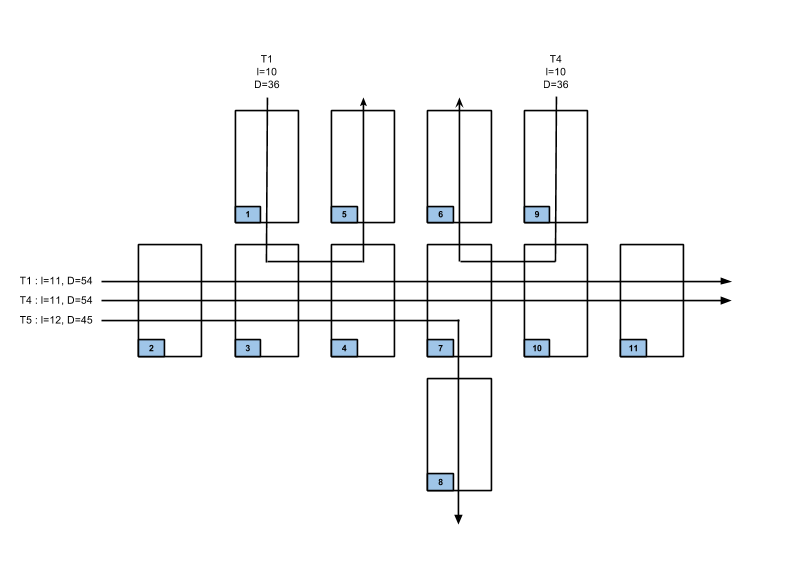
\includegraphics[width=\textwidth]{images/global.png}
  \center
  \caption{Schéma de l'example de la section 5 de l'article}
  \label{image_global}
\end{figureH}

\paragraph{}
$\tau_5$ ne peut pas être retardé à cause d'un flux de priorité supérieur. Par contre, il y a 3 flux qui peuvent retarder $\tau_5$ à cause de la non-préemption.
\[ R_{5} = [(5-1) \times 1]  + [5 \times 4] + [3 \times (4-1)] + [0] = 33 \]

\begin{figureH}
  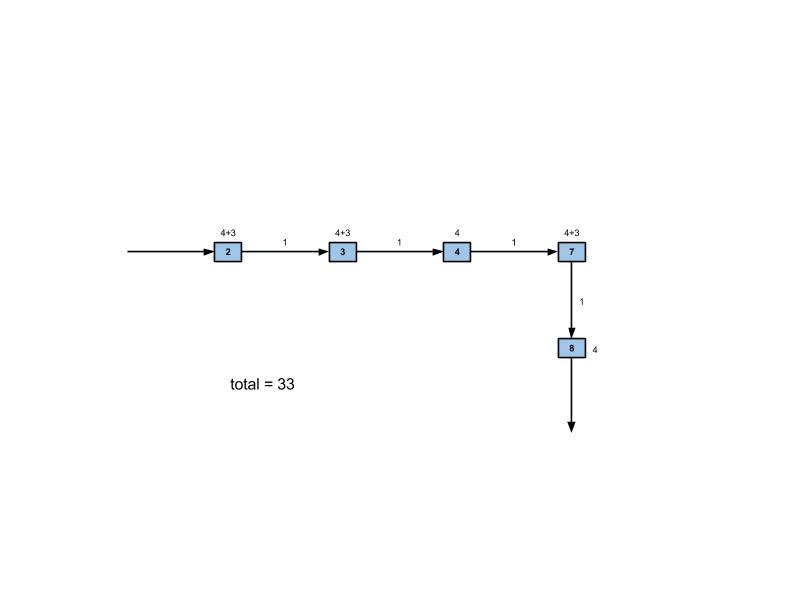
\includegraphics[width=\textwidth]{images/tache5.png}
  \center
  \caption{Chemin de la tache 5}
  \label{image_global}
\end{figureH}

\paragraph{}
$\tau_4$ et $\tau_3$ ont le même comportement. Ils peuvent être retardé à cause de la priorité supérieure de $\tau_5$. Ils peuvent se retarder entre eux. Ils peuvent être retardés à cause de la non-préemption de $\tau_1$ une fois au noeud 3 et à cause de la non-préemption de $\tau_2$ deux fois aux noeuds 7 et 10.
\[ R_{4} = R_3 = [(6-1) \times 1] +[ 6 \times 4] +[ 3 \times (4-1) ]+[ 4 + 4] = 46 \]

\begin{figureH}
  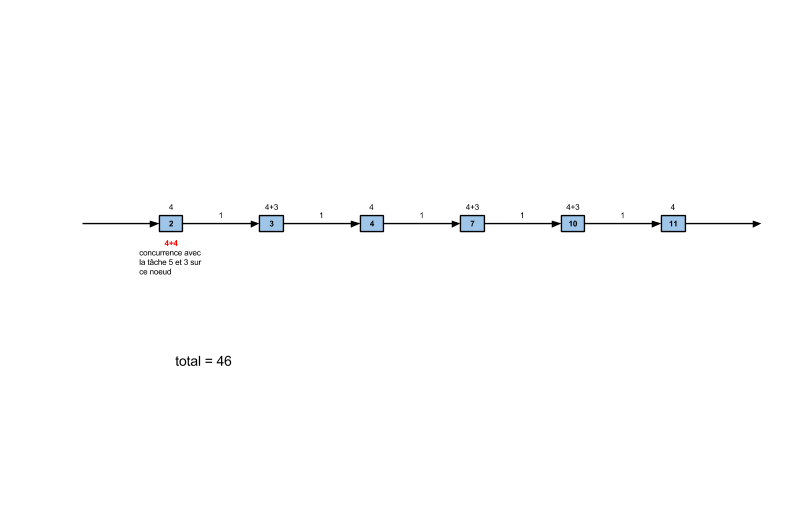
\includegraphics[width=\textwidth]{images/tache4.png}
  \center
  \caption{Chemin de la tache 4}
        \label{image_global}
\end{figureH}

\paragraph{}
$\tau_1$ peut être retardé à cause de la priorité supérieure de $\tau_5$, $\tau_4$ et $\tau_3$ au noeud 3. Par ailleurs, il n'existe pas de flux de priorité inférieure succeptible de retarder $\tau_1$ à cause de la non-préemption.
\[ R_1 = [(4-1)\times 1 ]+[ 4 \times 4] +[ 0] +[ 4 +4 +4] = 31 \]

\paragraph{}
$\tau_2$ peut dans le pire des cas être retardé une seule fois par $\tau_3$, $\tau_4$ et $\tau_5$ (car $T_i = 36$) soit au noeud 10 ou soit au noeud 7.
\[ R_2 = [(4-1) \times 1 ] + [4 \times 4 ] + [0] + [4+4+4] = 31\]


    



\end{document}
